\documentclass[compress]{beamer}
\usepackage{irbookslide}
\usepackage{irilmenau2}
\usepackage{tikz}
\usepackage{url}
\usepackage{ifxetex}
\RequireXeTeX
\usepackage{fontspec} % zahteva paket euenc
\usepackage{xunicode}
\usepackage{xltxtra}
\usepackage{polyglossia}
%\setdefaultlanguage[script=Latin]{serbian}

\title{Internet softverske arhitekture}
\subtitle{Slajdovi sa predavanja}
\author{Branko Milosavljević}
\institute{Katedra za informatiku, Fakultet tehničkih nauka, Univerzitet u
Novom Sadu}
\date{2014.}
\subject{Predavanja sa ISA}

\begin{document}

\frame{\titlepage}

\section{Predmet}
\frame{
  \frametitle{Sajt predmeta}
  \begin{center}
    \Large{\url{https://enastava.io}}
    \Large{\url{http://www.informatika.ftn.ns.ac.yu/ISA}}
  \end{center}
}
\frame{
  \frametitle{Ko drži nastavu}
  \begin{itemize}
    \item Branko Milosavljević, TMD 120 \\ \texttt{mbranko@uns.ac.rs}
    \item Igor Cverdelj-Fogaraši, TMD 15A \\ \texttt{igor.fogarasi@uns.ac.rs}
    \item Željko Ivković, TMD 16 \\ \texttt{zeljkoi@uns.ac.rs}
  \end{itemize}
}
\frame{
  \frametitle{Ispitne obaveze}
  \begin{itemize}
    \item Odbranjen projektni zadatak posle ovog semestra
    \begin{itemize}
      \item odbranjen projekat važi trajno
      \item mora se odbraniti do kraja sledećeg zimskog semestra; posle toga zadatak se menja
    \end{itemize}
    \item Usmeni ispit
  \end{itemize}
}
\frame{
  \frametitle{Literatura}
  \begin{itemize}
    \item R.P. Sriganesh, G. Brose, M. Silverman. {\em Mastering EJB 3.0}. Wiley, 2006.
    \item C. Bauer, G. King. {\em Java Persistence with Hibernate}. Manning, 2007.
    \item D. Panda, R. Rahman, D. Lane. {\em EJB 3.0 In Action}. Manning, 2007.
  \end{itemize}
}
\frame{
  \frametitle{Ovi slajdovi}
  \begin{itemize}
    \item Ovi slajdovi su samo pomoćni materijal
    \item (Verovatno) nisu dovoljni za polaganje ispita
  \end{itemize}
}

\section[RMI]{Tehnologije distribuiranih objekata}
\frame{
  \frametitle{Remote Method Invocation (RMI)}
  \begin{itemize}
    \item Osnovna tehnologija za rad sa distribuiranim objektima u Javi
    \item Objekti na udaljenim JVM su dostupni preko mreže
    \item Pozivamo njihove metode na isti način kao i za lokalne objekte
    \item Objekti se registruju u katalozima (registry)
    \item Klijenti ih tamo pronalaze
  \end{itemize}
}
\frame{
  \frametitle{RMI registry, server i klijent}
  \begin{center}
    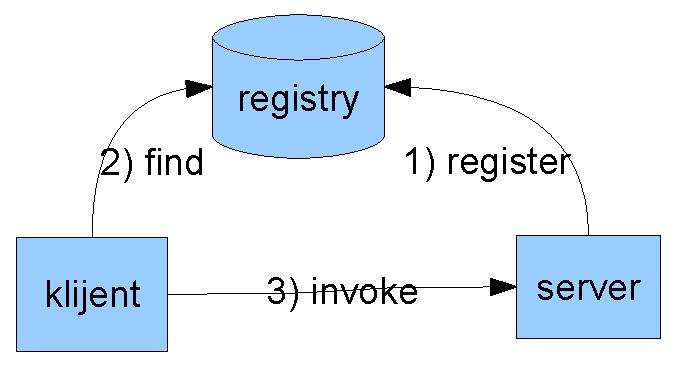
\includegraphics[width=10cm]{pic01.pdf}
  \end{center}
}
\frame{
  \frametitle{RMI klijent i server komuniciraju preko posrednika}
  \begin{center}
    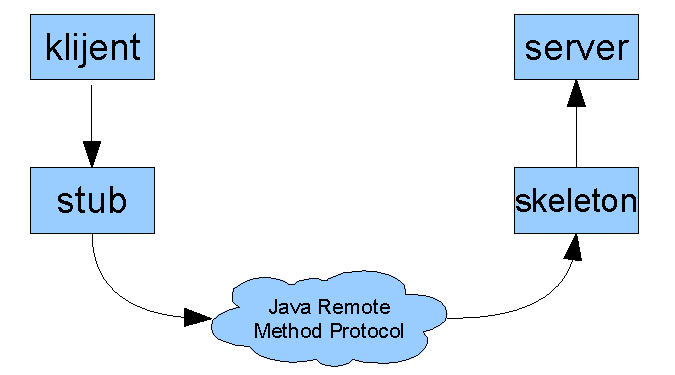
\includegraphics[width=10cm]{pic02.pdf}
  \end{center}
}
\frame{
  \frametitle{Primer elementarnog RMI klijenta i servera}
  \begin{itemize}
    \item Primer 1
  \end{itemize}
}
\frame{
  \frametitle{RMI i prenos programskog koda}
  \begin{itemize}
    \item Prilikom poziva metode RMI objekta...
    \item ...kao parametar možemo proslediti instancu klase koja nasleđuje tip parametra
    \item Tada će JVM preneti i programski kod potrebne klase!
    \item Primer 2
  \end{itemize}
}
\frame{
  \frametitle{JNDI}
  \begin{itemize}
    \item Java Naming and Directory Interface
    \item Standardni API za pristup različitim servisima imena
    \item I različitim direktorijumskim servisima
    \item Servis imena: mapira ime (string) $\leftrightarrow$ objekat
    \begin{itemize}
      \item Fajl-sistem
      \item RMI registry
    \end{itemize}
    \item Direktorijumski servis: objekti se dodatno opisuju pomoću atributa
    \begin{itemize}
      \item DNS
      \item LDAP / Active Directory / NDS...
    \end{itemize}
    \item Pristup različitim servisima obavlja se kroz isti API ali preko različitog ,,provajdera`` (tj. drajvera)
    \begin{itemize}
      \item analogno sa JDBC
    \end{itemize}
  \end{itemize}
}
\frame{
  \frametitle{JNDI}
  \begin{itemize}
    \item Primer 3
  \end{itemize}
}
\frame{
  \frametitle{RMI + JNDI}
  \begin{itemize}
    \item Umesto Naming.lookup() možemo da koristimo JNDI API za pronalaženje RMI objekta
    \item Primer 4
  \end{itemize}
}
\section{EJB3}
\frame{
\frametitle{Java EE}
\begin{itemize}
  \item Enterprise JavaBeans (EJB) 3.0 --- JSR-220
  \item JavaServer Pages (JSP) 2.1 --- JSR-245
  \item JavaServer Faces (JSF) 1.2 --- JSR-252
  \item JSP Standard Template Library (JSTL) 1.1 --- JSR-52
  \item Java API for XML Binding (JAXB) 2.0 --- JSR-222
  \item Java API for XML -- Web Services (JAX-WS) 2.0 --- JSR-224
  \item Web Service Annotations (WS Annotations) --- JSR-181
\end{itemize}
}
\frame{
  \frametitle{EJB 3.0}
  \begin{itemize}
    \item Programski model za pisanje distribuiranih komponenti
    \item Svrha komponenti:
    \begin{itemize}
      \item Vrše programsku obradu (implementiraju ,,poslovnu logiku``) ---
      \mygreen{session beans}
      \item Reprezentuju podatke u (relacionoj) bazi podataka --- \\
      \mygreen{entities}
      \item Vrše programsku obradu uz asinhrono pozivanje ---
      \mygreen{message-driven beans}
    \end{itemize}
    \item Distribuirane: dostupne preko mreže
  \end{itemize}
}
\frame{
  \frametitle{EJB 3.0}
  \begin{itemize}
    \item Temeljno prerađena specifikacija bazirana na prethodnim iskustvima
    \item Loša iskustva sa EJB 2.1
    \item Dobra iskustva iz različitih (open source) projekata
    \begin{itemize}
      \item Hibernate: O/R mapiranje ,,urađeno kako treba``
      \item Spring: životni ciklus, dependency injection, AOP
    \end{itemize}
    \item upotreba \mygreen{anotacija} eliminiše XML konfiguracione fajlove
  \end{itemize}
}
\section{Session beans}
\frame{
  \frametitle{EJB 3.0: Session bean}
  \begin{itemize}
    \item Session bean se sastoji iz
    \begin{itemize}
      \item remote i/ili lokalnog interfejsa
      \item bean klase
    \end{itemize}
    \item Klijent ga pronalazi pomoću JNDI-a
    \item i poziva njegove metode
  \end{itemize}
}
\frame{
  \frametitle{Dve vrste session beanova}
  \begin{itemize}
    \item \mygreen{Stateless}: ne pamti stanje između poziva svojih metoda
    \begin{itemize}
      \item bean klasa može imati atribute ali se ne garantuje za njihov sadržaj prilikom sledećeg poziva!
    \end{itemize}
    \item \mygreen{Stateful}: pamti stanje između poziva
  \end{itemize}
}
\frame{
  \frametitle{Stateless session bean}
  \begin{itemize}
    \item Primer 5
  \end{itemize}
}
\frame{
  \frametitle{Stateful session bean}
  \begin{itemize}
    \item Primer 6
  \end{itemize}
}
\frame{
  \frametitle{Stateless vs stateful: performanse}
  \begin{itemize}
    \item Stateless
    \begin{itemize}
      \item jednostavni za pooling, zaključavanje na nivou poziva metode
    \end{itemize}
    \item Stateful
    \begin{itemize}
      \item komplikovani za pooling, zaključavanje na nivou celog objekta
    \end{itemize}
  \end{itemize}
}
\frame{
  \frametitle{Životni ciklus session beana}
  \begin{center}
    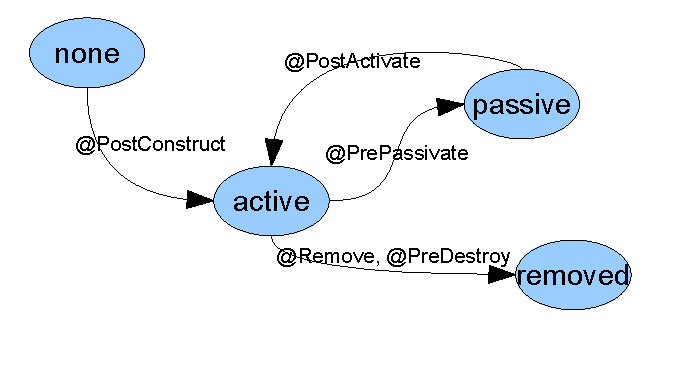
\includegraphics[width=10cm]{pic03.pdf}
  \end{center}
  \begin{itemize}
    \item Primer 7
  \end{itemize}
}
\frame{
  \frametitle{Session bean poziva drugi session bean}
  \begin{itemize}
    \item Prvi SB se ponaša kao klijent za drugi SB
    \item Ako se nalaze u istom kontejneru, može da koristi lokalni interfejs
    \item Pronalazi ga preko JNDI konteksta
    \item Inicijalni kontekst se konstruiše bez parametara
    \item Primer 8
  \end{itemize}
}
\section[DI]{Dependency injection}
\frame{
  \frametitle{Session bean i dependency injection}
  \begin{itemize}
    \item Drugi način da jedan SB dobije referencu na drugi je pomoću \mygreen{dependency injection} mehanizma
    \item Referencu na drugi SB upisuje {\bf kontejner} u atribut prvog SB
    \item Atribut je potrebno označiti anotacijom {\bf @EJB}
    \item Primer 9
  \end{itemize}
}
\frame{
  \frametitle{Session bean i dependency injection}
  \begin{itemize}
    \item Dependency injection je moguć u sledećim slučajevima \\ (bean A $\rightarrow$ (poziva) bean B)
    \begin{itemize}
      \item stateless $\rightarrow$ stateless
      \item stateful $\rightarrow$ stateless
      \item stateful $\rightarrow$ stateful
    \end{itemize}
    \item A zabranjen je u slučaju
    \begin{itemize}
      \item stateless $\rightarrow$ stateful
    \end{itemize}
  \end{itemize}
}
\frame{
  \frametitle{Session bean i dependency injection}
  \begin{itemize}
    \item Anotacijom {\bf @Resource} mogu da se označe atributi sledećeg tipa
    \begin{itemize}
      \item javax.ejb.SessionContext
      \item javax.sql.DataSource
      \item javax.transaction.UserTransaction
      \item javax.jms.Queue, javax.jms.Topic
      \item \ldots
    \end{itemize}
    \item Anotacijom {\bf @PersistenceContext} označava se atribut tipa
    \begin{itemize}
      \item javax.persistence.EntityManager
    \end{itemize}
    \item Anotacijom {\bf @PersistenceContextFactory} označava se atribut tipa
    \begin{itemize}
      \item javax.persistence.EntityManagerFactory
    \end{itemize}
  \end{itemize}
}
\section[AOP]{Elementi aspekt-orijentisanog programiranja}
\frame{
  \frametitle{Aspekt-orijentisano programiranje (AOP)}
  \begin{itemize}
    \item Sredstvo za izražavanje određenih pravila/procedura koja se mogu primeniti na više mesta u programu
    \item Npr. logovanje, kontrola pristupa, \ldots -- aspekti programa koji nisu direktno vezani za poslovnu logiku
      i često izgledaju isto za različite poslovne procedure
    \item \mygreen{Aspekt} je parče koda koji se može vezati za neku metodu tako da se izvrši
    \begin{itemize}
      \item pre poziva metode
      \item posle poziva metode
      \item oko poziva metode (obuhvata poziv)
    \end{itemize}
  \end{itemize}
}
\frame{
  \frametitle{Session beans i AOP}
  \begin{itemize}
    \item U EJB 3.0 aspekti mogu da {\bf obuhvate} poziv metode
    \item Metodu je potrebno označiti anotacijom {\bf @Interceptor}
    \item Ako ima više aspekata onda {\bf @Interceptors}
    \item Parametar ove anotacije je klasa koja sadrži aspekt
    \item Aspekt je metoda u klasi označena anotacijom {\bf @AroundInvoke}
    \item Primer 10
  \end{itemize}
}
\frame{
  \frametitle{Interceptori i životni ciklus beana}
  \begin{itemize}
    \item Klasa navedena kao @Interceptor može sadržati i metode za obaveštavanje o događajima u životnom ciklusu
    \item U primeru 7 te metode su bile deo bean klase
    \item Možemo ih premestiti u interceptor klasu
    \item Koristimo iste anotacije: @PostConstruct, @PrePassivate, @PostActivate, @PreDestroy
    \item Primer 11
  \end{itemize}
}
\section[JDBC]{Pristup relacionim bazama podataka}
\frame{
  \frametitle{Pristup relacionim bazama podataka}
  \begin{itemize}
    \item standardan API koji omogućava pristup relacionim bazama podataka --
    \textbf{JDBC}
    \item klase i interfejsi u paketu \texttt{java.sql}
    \item komunikacija putem SQL-a
    \item API implementira konkretna biblioteka za konkretnu bazu -- MySQL,
    Oracle, \ldots
    \item promena baze (npr. MySQL $\rightarrow$ PostgreSQL) ne [bi trebalo da]
    zahteva promenu našeg koda
  \end{itemize}
}
\begin{frame}[fragile]
  \frametitle{Korak 1: inicijalizacija drajvera}
\begin{verbatim}
Class.forName("com.mysql.jdbc.Driver");
\end{verbatim}
\end{frame}
\begin{frame}[fragile]
  \frametitle{Korak 2: otvaranje konekcije}
\begin{verbatim}
import java.sql.Connection;
...
Connection conn = DriverManager.getConnection(
  "jdbc:mysql://localhost/isa",   // JDBC URL
  "isa",                          // username
  "isa");                         // password
\end{verbatim}
\end{frame}
\begin{frame}[fragile]
  \frametitle{Korak 3a: kreiranje i izvršavanje SQL naredbe}
\begin{verbatim}
import java.sql.Statement;
...
Statement stmt = conn.createStatement();
stmt.executeUpdate(
  "INSERT INTO nastavnici ('Ana', 'Tot', 'docent'");
stmt.close();
\end{verbatim}
\end{frame}
\begin{frame}[fragile]
  \frametitle{Korak 3b: kreiranje i izvršavanje SQL upita}
\begin{verbatim}
import java.sql.Statement;
import java.sql.ResultSet;
...
Statement stmt = conn.createStatement();
ResultSet rset = stmt.executeQuery(
  "SELECT ime, prezime, zvanje FROM nastavnici");
while (rset.next()) {
  rset.getString(1); // ime
  rset.getString(2); // prezime
  rset.getString(3); // zvanje
}
rset.close();
stmt.close();
\end{verbatim}
\end{frame}
\begin{frame}[fragile]
  \frametitle{Korak 4: zatvaranje konekcije}
\begin{verbatim}
conn.close();
\end{verbatim}
  \begin{itemize}
    \item TCP konekcija je otvorena sve vreme dok je JDBC konekcija otvorena!
    \item konekciju držimo otvorenu sve vreme rada sa bazom podataka
    \item tipično se više naredbi se izvrši kroz jednu konekciju
  \end{itemize}
\end{frame}
\frame{
  \frametitle{Primer postavljanja upita}
  \begin{itemize}
    \item primer 12 $\rightarrow$ isa.pr12.Db1
  \end{itemize}
}
\frame{
  \frametitle{Ponavljanje istih SQL naredbi}
  \begin{itemize}
    \item izvršavanje SQL naredbe na serveru podrazumeva pripremne radnje
    \item parsiranje komande, kreiranje plana izvršavanja, itd.
    \item u slučaju ponovljenih istih komandi te pripremne radnje se takođe
    ponavljaju
    \item to je čist višak
  \end{itemize}
}
\frame{
  \frametitle{PreparedStatement}
  \begin{itemize}
    \item najavljuje serveru baze podataka izvršavanje jedne naredbe
    \item server obavlja pripremu za njeno izvršavanje
    \item šalje podatke za prvu 1. naredbe i izvršava je
    \item šalje podatke za prvu 2. naredbe i izvršava je
    \item šalje podatke za prvu 3. naredbe i izvršava je
    \item \ldots
    \item (znatno efikasnije!) \\ \ \\
    \item primer 12 $\rightarrow$ isa.pr12.Db2
  \end{itemize}
}
\frame{
  \frametitle{Uskladištene procedure}
  \begin{itemize}
    \item \mygreen{stored procedure} je potprogram napisan jeziku koji
    predstavlja proceduralno proširenje SQL-a
    \item može se pozvati sa klijenta
    \item njihova upotreba znatno smanjuje mrežni saobraćaj između klijenta i
    servera baze podataka
  \end{itemize}
}
\begin{frame}[fragile]
  \frametitle{Primer uskladištene procedure}
\begin{verbatim}
CREATE PROCEDURE povezi(
    IN ime_ VARCHAR(25), 
    IN prezime_ VARCHAR(35), 
    IN naziv_ VARCHAR(150))
BEGIN
  DECLARE nas_id INT;
  DECLARE pred_id INT;

  SELECT nastavnik_id INTO nas_id FROM nastavnici 
    WHERE ime=ime_ AND prezime=prezime_;
  SELECT predmet_id INTO pred_id FROM predmeti 
    WHERE naziv=naziv_;
  INSERT INTO predaje (nastavnik_id, predmet_id) 
    VALUES (nas_id, pred_id);
END//
\end{verbatim}
\end{frame}
\frame{
  \frametitle{Primer pozivanja uskladištene procedure}
  \begin{itemize}
    \item primer 12 $\rightarrow$ isa.pr12.Db3
  \end{itemize}
}
\frame{
  \frametitle{Pristup bazi podataka iz servleta}
  \begin{itemize}
    \item jedna instanca servleta opslužuje sve korisnike
    \item potencijalno više paralelnih niti
    \item otvaranje konekcije bi se moglo smestiti u \textbf{init()}
    \item zatvaranje konekcije u \textbf{destroy()} \\ \ \\
    \item primer 12 $\rightarrow$ isa.pr12.Db4
  \end{itemize}
}
\frame{
  \frametitle{Pristup bazi podataka iz servleta}
  \begin{itemize}
    \item jedna ista konekcija ne sme se koristiti u više paralelnih niti!
    \item trebaće nam po jedna konekcija \textbf{za svaku nit}
    \item \mygreen{resource pooling} slično kao za stateless bean-ove \\ \ \\
    \item primer 13 $\rightarrow$ klasa \textbf{ConnectionPool}
  \end{itemize}
}
\frame{
  \frametitle{JDBC je zamoran}
  \begin{itemize}
    \item naš Java program rukuje objektima
    \item podatke iz objekata treba ,,prepisati`` u tabele u bazi podataka
    \item JDBC API je opširan \\ \ \\
    \item primer 14
  \end{itemize}
}
\frame{
  \frametitle{JDBC je zamoran, i dalje}
  \begin{itemize}
    \item možemo da ,,sakrijemo`` JDBC pozive u klasu koja se snima u bazu
    \item korišćenje takve klase sada je jednostavnije 
    \item ali i dalje neko mora da napiše taj kod \\ \ \\
    \item primer 15
  \end{itemize}
}
\section[JPA]{Entitiji}
\frame{
  \frametitle{Java Persistence API (JPA)}
  \begin{itemize}
    \item Standardan API koji omogućava snimanje POJO objekata u relacionu bazu
    \item API implementira neka konkretna biblioteka -- Hibernate, TopLink, \ldots
    \item JPA-QL: upitni jezik, ,,objektna varijanta`` SQL-a
    \item O/R mapiranje se opisuje anotacijama
    \item Nema posebnih konfiguracionih fajlova (kao za klasičan Hibernate)
    \item JPA nije vezan za EJB kontejner -- može da se koristi i za Java SE aplikacije!
  \end{itemize}
}
\frame{
  \frametitle{Persistence Unit}
  \begin{itemize}
    \item \mygreen{Persistence unit} predstavlja jednu grupu perzistentnih klasa
    i parametara mapiranja
    \item Jedna aplikacija može raditi sa više persistence unita
    \item Persistence uniti se opisuju u fajlu META-INF/persistence.xml koji mora biti u CLASSPATH-u
  \end{itemize}
}
\frame{
  \frametitle{EntityManagerFactory}
  \begin{itemize}
    \item Na osnovu persistence unita opisanog XML fajlom u programu se kreira {\bf EntityManagerFactory}
    \item Predstavlja in-memory reprezentaciju O/R mapiranja
    \item Thread-safe klasa
    \item Kreiranje je skupo
  \end{itemize}
}
\frame{
  \frametitle{EntityManager}
  \begin{itemize}
    \item Komunikacija sa bazom odvija se u \mygreen{sesijama}
    \item Svaku sesiju opisuje jedan {\bf EntityManager} objekat
    \item Kreira ga EntityManagerFactory
    \item Nije thread-safe
    \item Kreiranje nije skupo
  \end{itemize}
}
\frame{
  \frametitle{EntityManager metode}
  \begin{itemize}
    \item void persist(Object entity)
    \item T merge(T entity)
    \item void remove(Object entity)
    \item T find(Class<T> entityClass, Object primaryKey)
    \item Query createQuery(String query)
    \item EntityTransaction getTransaction()
    \item close()
    \item \ldots
  \end{itemize}
}
\frame{
  \frametitle{JPA entity}
  \begin{itemize}
    \item \mygreen{Entity} je POJO klasa sa anotacijom {\bf @Entity}
    \item Mora imati default konstruktor
    \item Najčešće se mapira 1 klasa $\leftrightarrow$ 1 tabela
    \item Atributi klase se mapiraju na kolone tabele
    \item Parametri mapiranja se opisuju anotacijama
    \item Anotacije se vezuju za atribute ili getter metode
  \end{itemize}
}
\frame{
  \frametitle{JPA entity}
  \begin{itemize}
    \item Entity ne mora da implementira Serializable
    \item Ako ga implementira, entitiji se mogu prenositi u druge slojeve aplikacije
    \item Poseban DTO (Data Transfer Object) nije potreban
  \end{itemize}
}
\frame{
  \frametitle{JPA entity}
  \begin{itemize}
    \item Primer 16
    \begin{itemize}
      \item AdminTest: primer rukovanja entitijem pomoću EntityManagera
      \item Admin: primer entity klase
      \item persistence.xml: definicija persistence unita
    \end{itemize}
  \end{itemize}
}
\frame{
  \frametitle{Identitet u Javi}
  \begin{itemize}
    \item Identitet objekta (lokacija u memoriji): \texttt{x == y}
    \item Jednakost objekata: \texttt{x.equals(y)}
    \begin{itemize}
      \item da li su jednaka dva \texttt{User} objekta sa istim \texttt{username} a različitim \texttt{password}?
    \end{itemize}
  \end{itemize}
}
\frame{
  \frametitle{Identitet u bazi podataka}
  \begin{itemize}
    \item Isti red (lokacija na disku)
    \item Vrednost primarnog ključa
  \end{itemize}
}
\frame{
  \frametitle{Java identitet vs DB identitet}
  \begin{itemize}
    \item Kada je Java identitet $\Leftrightarrow$ DB identitet?
    \item Kada je Java jednakost $\Leftrightarrow$ DB jednakost?
  \end{itemize}
}
\frame{
  \frametitle{Primer 1}
  \begin{itemize}
    \item U prvoj transakciji: \\ \texttt{x = em.find(User.class, "mbranko");}
    \item U drugoj transakciji: \\ \texttt{y = em.find(User.class, "mbranko");}
    \item Da li je \texttt{x == y} ?
  \end{itemize}
}
\frame{
  \frametitle{Primer 2}
  \begin{itemize}
    \item U prvoj transakciji: \\ \texttt{x = em.find(User.class, "mbranko");}
    \item U drugoj transakciji: \\ \texttt{y = em.find(User.class, "mbranko");\\ y.setPassword("trt");}
    \item Da li je \texttt{x.equals(y)} ?
  \end{itemize}
}
\frame{
  \frametitle{JPA sesija}
  \begin{itemize}
    \item Java identitet (i jednakost) važi za perzistentne objekte \textbf{unutar jedne sesije}! \\
      \texttt{EntityManager em = emf.createEntityManager(); \\
      \ldots \\
      em.close();}
  \end{itemize}
}
\frame{
  \frametitle{Životni ciklus entitija}
  \begin{center}
    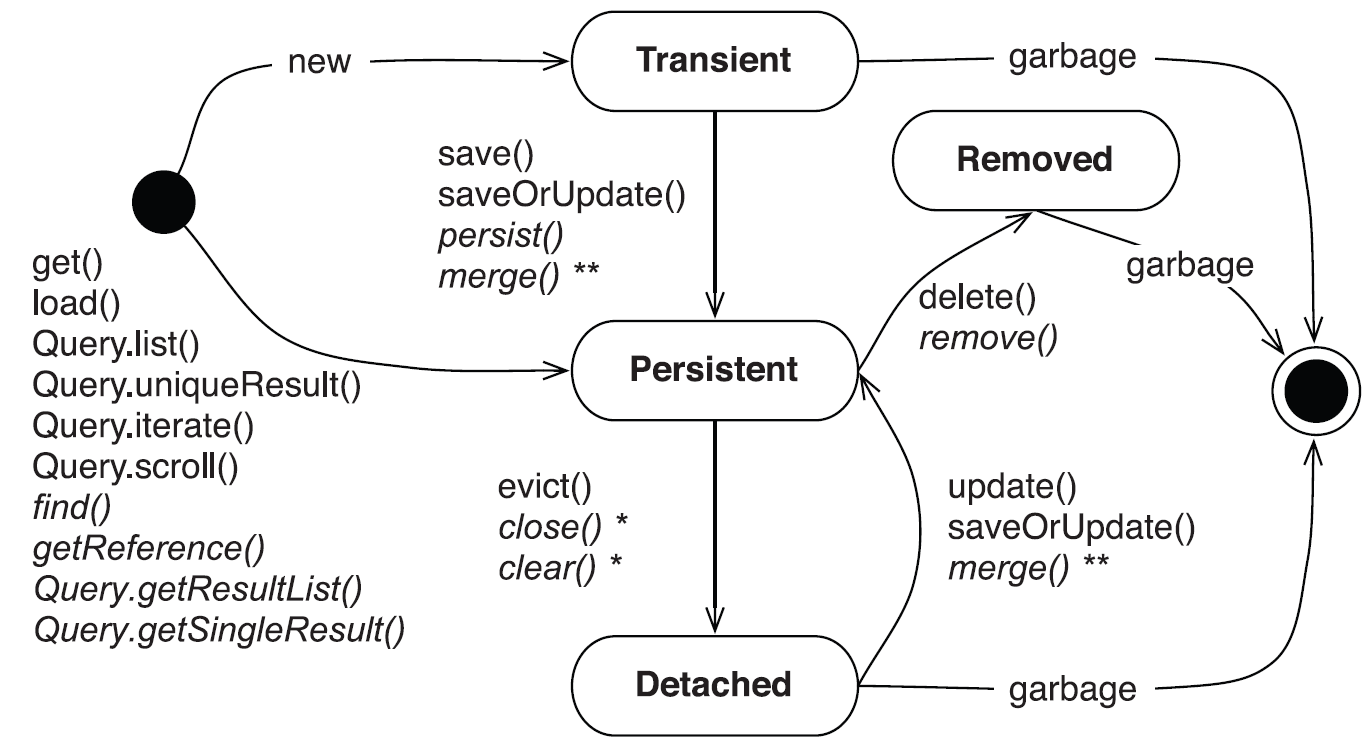
\includegraphics[width=10cm]{pic14.png}
  \end{center}
}
\section[Veze]{Veze između entitija}
\frame{
  \frametitle{Tipovi veza između entitija}
  \begin{itemize}
    \item Posmatramo dve klase, A i B, koje su u vezi
    \item Veza tipa 1:1
    \begin{itemize}
      \item klasa A sa atributom tipa B, anotacija @OneToOne
      \item klasa B sa atributom tipa A, anotacija @OneToOne
    \end{itemize}
    \item Veza tipa 1:n
    \begin{itemize}
      \item 1-strana ima anotaciju @OneToMany, tip atributa je Set<B>
      \item n-strana ima anotaciju @ManyToOne, tip atributa je A
      \item n-strana obično ima i anotaciju @JoinColumn koja opisuje join uslov
    \end{itemize}
    \item Veza tipa m:n
    \begin{itemize}
      \item m-strana ima anotaciju @ManyToMany, tip atributa je Set<B>
      \item n-strana ima anotaciju @ManyToMany, tip atributa je Set<A>
      \item opciono i @JoinColumn
    \end{itemize}
  \end{itemize}
}
\frame{
  \frametitle{Jedno- i dvosmerne veze}
  \begin{itemize}
    \item Jednosmerna veza: klasa A ,,vidi`` klasu B, a klasa B ,,ne vidi`` klasu A
    \item Dvosmerna veza: klasa A ,,vidi`` klasu B i obrnuto
    \item Prethodni slajd podrazumeva dvosmernu vezu
    \item Jednosmernu vezu pravimo izostavljanjem odgovarajućeg atributa u klasi
  \end{itemize}
}
\begin{frame}[fragile]
  \frametitle{Uspostavljanje veze}
  \begin{itemize}
    \item Važno pravilo: uspostavljanje veze između objekata mora da se vrši {\bf kao da se ne koristi JPA}
    \item Ako je dvosmerna, veza mora da se ažurira sa obe strane
  \end{itemize}
\begin{verbatim}
// oba reda su obavezna
product.setCategory(category);
category.getProducts().add(product);
\end{verbatim}
\end{frame}
\begin{frame}[fragile]
  \frametitle{Inicijalizacija atributa}
  \begin{itemize}
    \item Atribut tipa Set<X> se mora inicijalizovati u prilikom konstrukcije objekta
    \item Obično se za inicijalizaciju koristi HashSet<X>
    \item JPA engine će taj kasnije taj objekat zameniti svojom Set implementacijom
  \end{itemize}
\begin{verbatim}
class Category {
  ...
  private Set<Product> products = new HashSet<Product>();
  ...
}
\end{verbatim}
\end{frame}
\frame{
  \frametitle{Primer 17}
  \begin{center}
    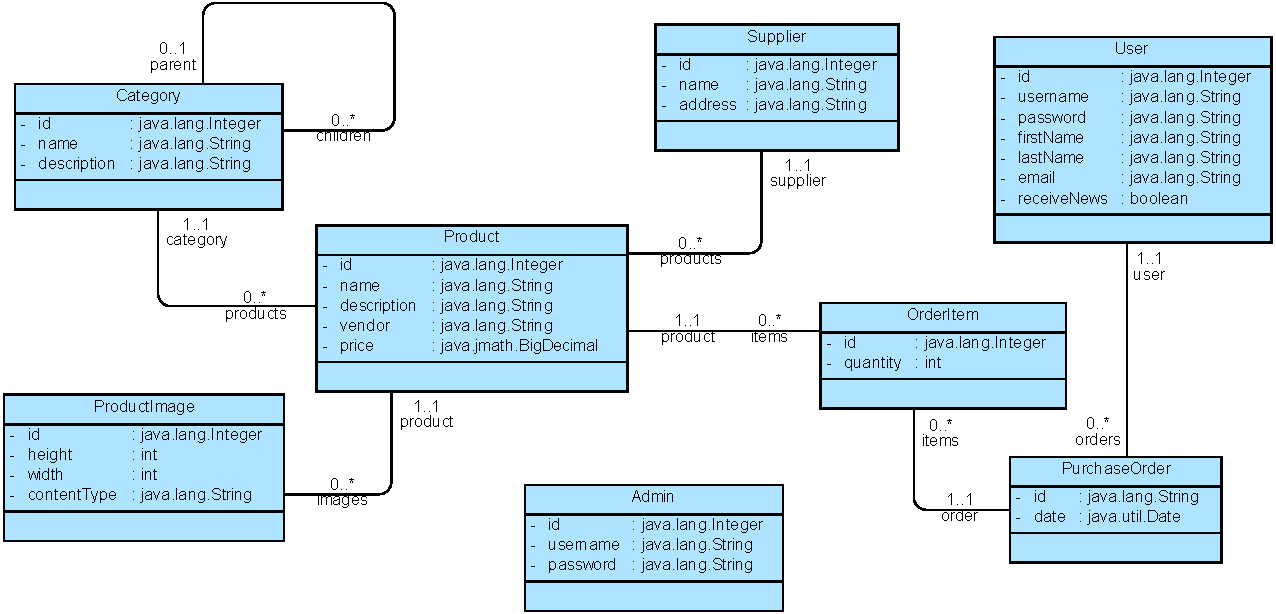
\includegraphics[width=11.5cm]{pic04.pdf}
  \end{center}
}
\frame{
  \frametitle{Dodavanje novog elementa u Set}
  \begin{itemize}
    \item Set ne prihvata duplikate
    \item Prilikom dodavanja novog elementa, proverava se da li je element već tamo
    \item Provera se oslanja na \texttt{equals()} i \texttt{hashCode()}
    \item ...a oni su nasleđeni iz klase \texttt{Object} i ne rade kako treba!
  \end{itemize}
}
\begin{frame}[fragile]
  \frametitle{equals() za entitije}
  \begin{itemize}
    \item \texttt{Object.equals()} $\Leftrightarrow$ \texttt{==}
    \item Dva različita objekta u memoriji mogu predstavljati isti red u bazi!
    \item Treba redefinisati \texttt{equals()} tako da koristi primarni ključ u poređenju
  \end{itemize}
\begin{verbatim}
public boolean equals(Object o) {
  return this.id.equals(o.id);
}
\end{verbatim}
  \begin{itemize}
    \item<2-> Međutim, \texttt{id} nije definisan pre nego što se objekat snimi u bazu!
  \end{itemize}
\end{frame}
\begin{frame}[fragile]
  \frametitle{equals() za entitije}
  \begin{itemize}
    \item Dodatak: ako je \texttt{id == null} za bilo koji od dva objekta, smatramo da su različiti
  \end{itemize}
\begin{verbatim}
public boolean equals(Object that) {
  if (this == that) 
    return true;
  if (this.id == null || that.id == null)
    return false;
  return this.id.equals(other.id);
}
\end{verbatim}
  \begin{itemize}
    \item<2-> Sledeći problem: ako su dva objekta jednaka, moraju imati isti \texttt{hashCode()}
    \item<2-> Pri tome vrednost \texttt{hashCode()} ne sme da se menja -- izgubićemo objekte u Setu
  \end{itemize}
\end{frame}
\begin{frame}[fragile]
  \frametitle{hashCode() za entitije}
\begin{verbatim}
private Integer hashcodeValue = null;
public int hashCode(){
  if (hashcodeValue == null) {
    if (id == null)
      hashcodeValue = new Integer(super.hashCode());
    else
      hashcodeValue = id;
  }
  return hashcodeValue.intValue();
}
\end{verbatim}
  \begin{itemize}
    \item Kada se jednom upotrebi \texttt{hashCode()}, više se neće menjati
    \item<2-> Problem: napravimo novi objekat, snimimo ga, zatvorimo sesiju, kasnije učitamo objekat u novoj sesiji 
      i dobijemo dva objekta za koje važi \texttt{a.equals(b)} ali je \\ \texttt{a.hashCode() != b.hashCode()}
  \end{itemize}
\end{frame}
\begin{frame}[fragile]
  \frametitle{Drugo rešenje za equals() i hashCode()}
  \begin{itemize}
    \item Za poređenje koristimo one atribute koji su po svojoj prirodi jedinstveni
    \item Npr. za klasu \texttt{User} atribut \texttt{username} je jedinstven i \textbf{ne menja se nakon što se inicijalizuje}
      (tj. korisnik ne može da promeni svoj username kada se jednom registruje)
  \end{itemize}
\begin{verbatim}
public int hashCode(){
  return username.hashCode();
}
public boolean equals(Object that) {
  if (this == that)
    return true;
  if (that == null)
    return false;
  return this.username.equals(that.username);
}
\end{verbatim}
  \begin{itemize}
    \item<2-> Šta da radimo kad u klasi nema ovakvih atributa?
  \end{itemize}
\end{frame}
\begin{frame}[fragile]
  \frametitle{Idealno rešenje za equals() i hashCode()}
  \begin{itemize}
    \item Ne postoji
    \item Sve zavisi od načina upotrebe entitija
    \item Ako imamo atribut(e) sa jedinstvenim vrednostima, druga varijanta je najbolja
    \item Ako ih nemamo, prva varijanta može biti dovoljno dobra
    \item Treća varijanta: ne redefiniši \texttt{equals()} i \texttt{hashCode()} i pazi šta radiš
    \item Četvrta varijanta: GUID koji se inicijalizuje kod kreiranja objekta i koristi za 
            \texttt{equals()} i \texttt{hashCode()} -- može kao dodatni atribut ili čak primarni ključ
    \item Dobra diskusija: \url{http://www.hibernate.org/109.html}
  \end{itemize}
\end{frame}
\section[Webapps]{Struktura web aplikacija}
\frame{
  \frametitle{Pozivanje session beanova iz servleta}
  \begin{itemize}
    \item Servlet može da uradi JNDI lookup i pronađe session bean
    \item A može da koristi i dependency injection
    \item Servlet je po prirodi stateless, pa nema smisla injektovati stateful
    beanove \\ \ \\
    \item Primer 18
  \end{itemize}
}
\frame{
  \frametitle{Arhitektura web aplikacije koja koristi EJB}
  \begin{itemize}
    \item Klijent: servleti+JSP stranice
    \item Servleti pristupaju session beanovima
    \begin{itemize}
      \item SLSB se injektuje u atribut servleta
      \item SFSB se pronađe preko JNDI i smesti u HttpSession
    \end{itemize}
    \item Session beanovi pristupaju entitijima preko EntityManagera
    \begin{itemize}
      \item EntityManager se injektuje u atribut SB-a
    \end{itemize}
  \end{itemize}
}
\begin{frame}
  \frametitle{Data Access Object (DAO) sloj}
  \begin{itemize}
    \item U praksi su za svaki entity potrebne uobičajene CRUD (create, retrieve, update, delete) operacije
    \item Njih obično implementiraju posebne DAO klase
    \item Jedan entity -- jedan DAO
    \item Ima dosta ,,pešačkog`` posla
  \end{itemize}
\end{frame}
\begin{frame}[fragile]
  \frametitle{Generički DAO: implementacija zajedničkih operacija}
\begin{verbatim}
public interface GenericDao<T, ID extends Serializable> {
  public Class<T> getEntityType();
  public T findById(ID id);
  public List<T> findAll();
  public List<T> findBy(String query);
  public T persist(T entity);
  public T merge(T entity);
  public void remove(T entity);
  public void flush();
  public void clear();
}
\end{verbatim}
\end{frame}
\begin{frame}[fragile,shrink=10]
  \frametitle{Generički DAO: implementacija zajedničkih operacija}
\begin{verbatim}
public abstract class GenericDaoBean<T, ID extends Serializable> 
    implements GenericDao<T, ID> {
  ...
  
  @PersistenceContext
  protected EntityManager em;
  ...
}
\end{verbatim}
\end{frame}
\begin{frame}[fragile,shrink=10]
  \frametitle{Konkretni DAO za entity User}
\begin{verbatim}
public interface UserDao extends GenericDao<User, Integer> {
  public User login(String username, String password);
}


@Stateless
@Local(UserDao.class)
public class UserDaoBean extends GenericDaoBean<User, Integer> 
    implements UserDao {

  public User login(String username, String password) { ... }
}
\end{verbatim}
\end{frame}
\begin{frame}
  \frametitle{Primer 19}
  \begin{itemize}
    \item Entity klase --- isa.pr19.entity.*
    \item DAO klase --- isa.pr19.dao.*
    \item SB klase --- isa.pr19.session.*
    \item servleti --- isa.pr19.servlet.*
    \item JSP stranice --- isa.pr19.*
  \end{itemize}
\end{frame}

\section[TX]{Upravljanje transakcijama}
\frame{
  \frametitle{Transakcije i konkurentni pristup podacima}
  \begin{itemize}
    \item Prilikom istovremenog pristupa podacima može da dođe do štetnog preplitanja rada više transakcija
    \item Tom prilikom može da se javi više problema
  \end{itemize}
}
\frame{
  \frametitle{Lost update}
  \begin{itemize}
    \item \mygreen{Lost update}: dve transakcije menjaju isti podatak bez zaključavanja
  \end{itemize}
  \begin{center}
    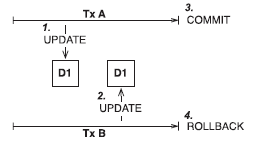
\includegraphics[width=6cm]{pic05.png}
  \end{center}
}
\frame{
  \frametitle{Dirty read}
  \begin{itemize}
    \item \mygreen{Dirty read}: transakcija A čita podatke pre nego što su commit-ovani
  \end{itemize}
  \begin{center}
    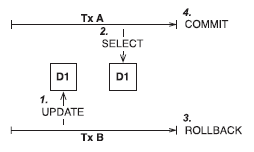
\includegraphics[width=6cm]{pic06.png}
  \end{center}
}
\frame{
  \frametitle{Unrepeatable read}
  \begin{itemize}
    \item \mygreen{Unrepeatable read}: transakcija A dva puta čita iste podatke i dobija različiti sadržaj
  \end{itemize}
  \begin{center}
    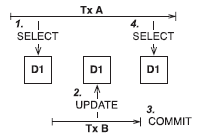
\includegraphics[width=6cm]{pic07.png}
  \end{center}
}
\frame{
  \frametitle{Phantom read}
  \begin{itemize}
    \item \mygreen{Phantom read}: transakcija A u drugom čitanju dobija i podatke kojih nije bilo prilikom prvog čitanja
  \end{itemize}
  \begin{center}
    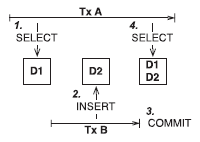
\includegraphics[width=6cm]{pic08.png}
  \end{center}
}
\begin{frame}[fragile]
  \frametitle{Transakcije na nivou JDBC konekcije}
  \begin{itemize}
    \item Transakcijama upravlja baza podataka
    \item Možemo da biramo nivo izolacije transakcija za svaku konekciju
    \item connection.setTransactionIsolation(...)
  \end{itemize}

  \begin{tabular}{l|l}
    \textbf{Nivo izolacije} & \textbf{Eliminiše problem} \\ \hline
    READ\_UNCOMMITTED & lost update \\
    READ\_COMMITTED & dirty read \\
    REPEATABLE\_READ & unrepeatable read \\
    SERIALIZABLE & phantom read
  \end{tabular}
\end{frame}
\begin{frame}
  \frametitle{Ko upravlja transakcijama kod EJB komponenti?}
  \begin{itemize}
    \item \mygreen{container-managed} tx: transakcijama upravlja kontejner na osnovu anotacija dodeljenih metodama
    \item \mygreen{bean-managed} tx: transakcijama programski upravlja bean (JTA API)
    \item \mygreen{client-managed} tx: transakcijama programski upravlja klijent (JTA API)
  \end{itemize}
\end{frame}
\begin{frame}
  \frametitle{Container-managed transakcije}
  \begin{itemize}
    \item Anotacija {\bf @TransactionAttribute}
  \end{itemize}
  \small{
  \begin{tabular}{l|l}
    \textbf{Vrednost} & \textbf{Značenje} \\ \hline
    REQUIRED & metoda se priključuje tekućoj tx, \\
      & otvara novu ako tx ne postoji \\ \hline
    REQUIRES\_NEW & metoda uvek pokreće novu tx, \\
      & ako postoji tekuća tx ona se suspenduje \\ \hline
    MANDATORY & metoda mora da se izvršava u tx, koja mora biti \\
      & ranije pokrenuta; ako je nema javlja se greška \\ \hline
    SUPPORTS & metoda će se priključiti tekućoj tx, ako ona postoji; \\ 
      & ako ne postoji, izvršava se bez tx \\ \hline
    NOT\_SUPPORTED & metoda se izvršava bez tx, \\ 
      & čak i ako postoji tekuća tx \\ \hline
    NEVER & metoda se izvršava bez tx; \\
      & ako postoji tekuća tx, javlja se greška
  \end{tabular}
  }
\end{frame}
\begin{frame}
  \frametitle{Container-managed transakcije}
  \begin{itemize}
    \item Primer 20: isa.pr20.container.*
  \end{itemize}
\end{frame}
\begin{frame}
  \frametitle{Bean-managed transakcije}
  \begin{itemize}
    \item Class-level anotacija \textbf{@TransactionManagement(BEAN)}
    \item Injekcija UserTransaction objekta pomoću @Resource anotacije
    \item Ručno pozivanje metoda
    \begin{itemize}
      \item UserTransaction.begin()
      \item UserTransaction.commit()
      \item UserTransaction.rollback()
    \end{itemize}
    \item Primer 20: isa.pr20.bean.*
  \end{itemize}
\end{frame}
\begin{frame}
  \frametitle{Client-managed transakcije}
  \begin{itemize}
    \item Klijent dobija UserTransaction preko JNDI lookup-a
    \item UserTransaction tx = (UserTransaction)ctx.lookup("java:comp/UserTransaction");
    \item Ručno pozivanje metoda
    \begin{itemize}
      \item tx.begin()
      \item tx.commit()
      \item tx.rollback()
    \end{itemize}
    \item Primer 20: isa.pr20.client.*
    \item (Beanovi koji se pozivaju su označeni kao bean-managed tx)
  \end{itemize}
\end{frame}
\frame{
  \frametitle{Optimističko i pesimističko zaključavanje}
  \begin{itemize}
    \item Problem: operacija B će pregaziti izmene koje napravi operacija A, ne znajući za njih
  \end{itemize}
  \begin{center}
    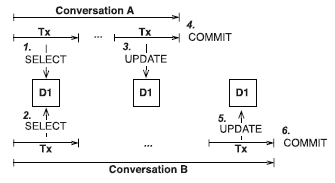
\includegraphics[width=8cm]{pic09.png}
  \end{center}
}
\begin{frame}
  \frametitle{Optimističko i pesimističko zaključavanje}
  \begin{itemize}
    \item Rešenje 1 -- \mygreen{pesimističko zaključavanje}: svaka operacija treba da zaključa podatke \textbf{i za čitanje i za pisanje} sve dok se ne završi
    \begin{itemize}
      \item u prethodnom primeru operacija B bi bila blokirana sve dok A ne otključa podatke
    \end{itemize}
    \item Rešenje 2 -- \mygreen{optimističko zaključavanje}: svaka operacija pre izmene podataka treba da proveri da li je podatke neko drugi u međuvremenu menjao
    \begin{itemize}
      \item poredi verziju podataka koje je pročitala sa onim što se trenutno nalazi u bazi
      \item ovo poređenje mora da se izvodi u režimu pesimističkog zaključavanja
      \item ako su podaci menjani, prijavi se greška korisniku
    \end{itemize}
  \end{itemize}
\end{frame}
\begin{frame}
  \frametitle{Optimističko i pesimističko zaključavanje}
  \begin{itemize}
    \item Pesimističko zaključavanje garantuje ispravan rad
    \item Ali ima loše performanse
    \begin{itemize}
      \item čak i ako dve transakcije pristupaju različitim redovima u tabeli može doći do blokiranja
    \end{itemize}
    \item Optimističko zaključavanje polazi od pretpostavke da u praksi do kolizije dolazi jako retko
    \begin{itemize}
      \item a situacije kada dođe do kolizije se otkrivaju i kontrola se vraća korisniku
    \end{itemize}
  \end{itemize}
\end{frame}
\begin{frame}
  \frametitle{Implementacija optimističkog zaključavanja}
  \begin{itemize}
    \item Varijanta 1: poredimo sve vrednosti objekta sa vrednostima u bazi
    \begin{itemize}
      \item nezgodno ako tabela ima puno kolona
    \end{itemize}
    \item Varijanta 2: dodamo novu kolonu koja služi kao brojač izmena
    \begin{itemize}
      \item na svaku izmenu u datom redu tabele inkrementiramo njenu vrednost
    \end{itemize}
  \end{itemize}
\end{frame}
\begin{frame}
  \frametitle{Optimističko zaključavanje i JPA}
  \begin{itemize}
    \item Implementacija pomoću ,,varijante 2``
    \item Entity dobija još jedan atribut tipa int koji se označava anotacijom \textbf{@Version}
    \item Atribut se mapira na novu kolonu u tabeli
    \item Ako dođe do kolizije generiše se OptimisticLockException
    \item Primer 21 -- isa.pr21.optimistic.*
  \end{itemize}
\end{frame}
\begin{frame}
  \frametitle{Pesimističko zaključavanje i JPA}
  \begin{itemize}
    \item Učitani entity može da se zaključa za čitanje pomoću EntityManagera:
    \item em.lock(entity, READ);
    \item Entity je zaključan do kraja transakcije
    \item Druga transakcija koja proba da zaključa objekat dobiće izuzetak
    \item Primer 21 -- isa.pr21.pessimistic.*
  \end{itemize}
\end{frame}

\section[Nasleđivanje]{Mapiranje nasleđivanja}
\begin{frame}
  \frametitle{Četiri varijante mapiranja nasleđivanja}
  \begin{itemize}
    \item Jedna tabela po konkretnoj klasi sa implicitnim polimorfizmom
    \item Jedna tabela po konkretnoj klasi
    \item Jedna tabela po hijerarhiji nasleđivanja
    \item Jedna tabela za svaku klasu
  \end{itemize}
\end{frame}
\begin{frame}
  \frametitle{1 tabela po konkretnoj klasi sa implicitnim polimorfizmom}
  \begin{center}
    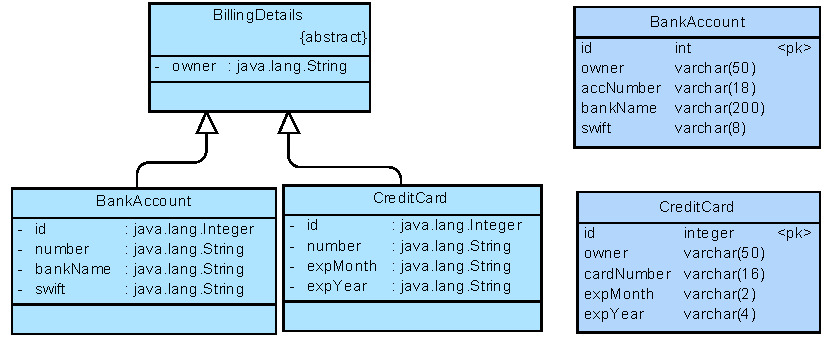
\includegraphics[width=9cm]{pic10.pdf}
  \end{center}
  \begin{itemize}
    \item Primer 22 -- isa.pr22.v1.*
  \end{itemize}
\end{frame}
\begin{frame}
  \frametitle{Jedna tabela po konkretnoj klasi}
  \begin{center}
    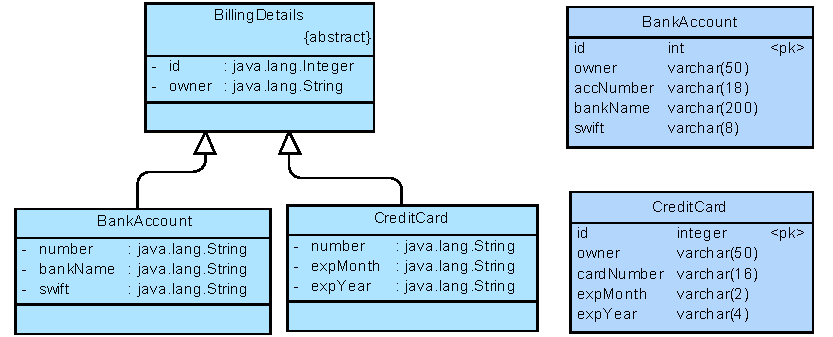
\includegraphics[width=9cm]{pic11.pdf}
  \end{center}
  \begin{itemize}
    \item Primer 22 -- isa.pr22.v2.*
  \end{itemize}
\end{frame}
\begin{frame}
  \frametitle{Jedna tabela po hijerarhiji nasleđivanja}
  \begin{center}
    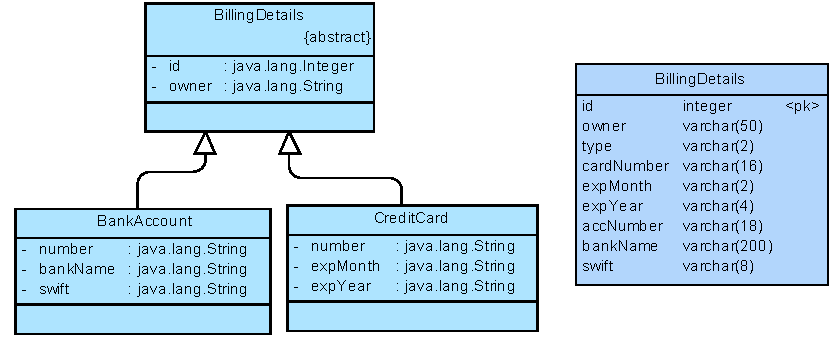
\includegraphics[width=9cm]{pic12.pdf}
  \end{center}
  \begin{itemize}
    \item Primer 22 -- isa.pr22.v3.*
  \end{itemize}
\end{frame}
\begin{frame}
  \frametitle{Jedna tabela za svaku klasu}
  \begin{center}
    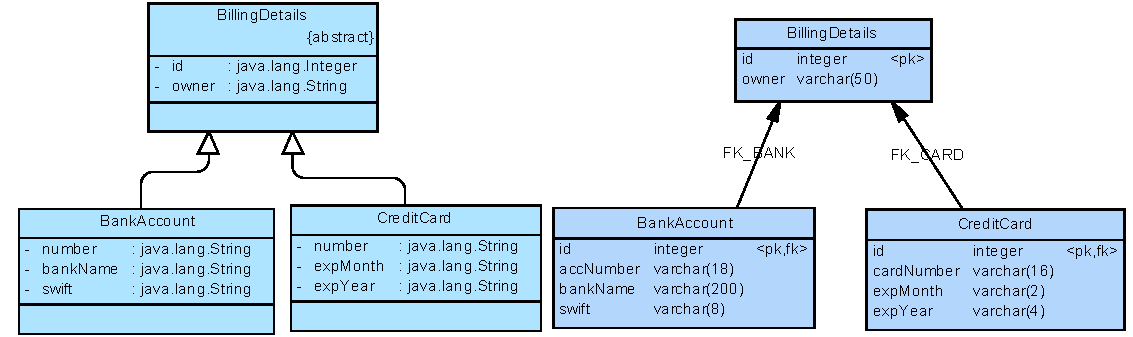
\includegraphics[width=11cm]{pic13.pdf}
  \end{center}
  \begin{itemize}
    \item Primer 22 -- isa.pr22.v4.*
  \end{itemize}
\end{frame}

\section[Ključevi]{Generisanje vrednosti primarnog ključa}
\begin{frame}
  \frametitle{Šta biramo za primarni ključ?}
  \begin{itemize}
    \item Neko prirodno obeležje koje je jedinstveno i nepromenljivo -- \mygreen{prirodni ključ}
    \begin{itemize}
      \item JMBG, PIO broj, \ldots
      \item može i grupa obeležja, npr. kontni okvir: šifra klase + šifra grupe + ...
    \end{itemize}
    \item Veštačko obeležje koje je jedinstveno -- \mygreen{surogatni ključ}
    \begin{itemize}
      \item integer brojač, UUID, \ldots
      \item ključ čini uvek jedno obeležje
    \end{itemize}
  \end{itemize}
\end{frame}
\begin{frame}
  \frametitle{Prirodni vs surogatni ključ}
  \begin{itemize}
    \item Prirodni ključevi
    \small{\begin{tabular}{l}
      \textbf{za} \\ \hline
      ne mora se izmišljati novo obeležje \\ %\hline
      \textbf{protiv} \\ \hline
      obeležje nije baš nepromenljivo \\
      ne mora biti integer tipa  $\rightarrow$ manje efikasno indeksiranje 
    \end{tabular}}
    \item Surogatni ključevi
    \small{\begin{tabular}{l}
      \textbf{za} \\ \hline
      efikasno indeksiranje \\ 
      nema više od jednog obeležja u ključu \\ %\hline
      \textbf{protiv} \\ \hline
      vrednost nema drugi smisao osim da bude jedinstvena
    \end{tabular}}
  \end{itemize}
\end{frame}
\begin{frame}
  \frametitle{Prirodni i surogatni ključevi i JPA}
  \begin{itemize}
    \item Za JPA se preporučuje upotreba surogatnih ključeva
    \item Znatno jednostavnije mapiranje
    \item Jednostavna provera da li treba raditi update (ključ $\neq$ null) ili insert (ključ = null)
  \end{itemize}

  \begin{itemize}
    \item Podržani su i prirodni ključevi
    \item Manje efikasan rad
    \item Manje elegantan objektni model u slučaju kompozitnih ključeva
  \end{itemize}
\end{frame}
\begin{frame}
  \frametitle{Generisanje vrednosti surogatnih ključeva}
  \begin{itemize}
    \item Identity / auto\_increment / \ldots kolona u bazi
    \item Sekvenca
    \item Tabela sa brojačima \\
    \small{\begin{tabular}{l|r}
      \textbf{counter\_name} & \textbf{counter\_value} \\ \hline
      users & 731 \\ 
      products & 8432 \\
      \ldots & \ldots
    \end{tabular}}
  \end{itemize}

  \begin{itemize}
    \item Primer 23 -- isa.pr23.surrogate.*
  \end{itemize}
\end{frame}
\begin{frame}
  \frametitle{JPA i prirodni ključevi}
  \begin{itemize}
    \item Ako prirodni ključ čini jedno obeležje, on se označava sa @Id, kao i ranije
    \item Ako ima više obeležja u ključu, mora se napraviti posebna ,,PK`` klasa
    \item Atribut tipa PK klase se dodaje u osnovnu klasu i označava sa @EmbeddedId
  \end{itemize}

  \begin{itemize}
    \item Spoljni ključ koji se sastoji iz više obeležja se opisuje @JoinColumns anotacijom
    \item Osim ako je spoljni ključ deo primarnog ključa -- tada se izražava u PK klasi
    \item Objektni model više nije elegantan!
  \end{itemize}

  \begin{itemize}
    \item Primer 23 -- isa.pr23.natural.*
  \end{itemize}
\end{frame}

\section[MDB]{Message-driven beans i JMS}
\begin{frame}
  \frametitle{Message-driven beans}
  \begin{itemize}
    \item Komponente koje se pozivaju asinhrono -- ne čeka se na rezultat izvršavanja
    \item Komunikacija klijenta i MDBa se odvija putem poruka
    \item Klijent šalje poruke MDBu, ovaj ih obrađuje kada stigne
  \end{itemize}

  \begin{itemize}
    \item MDB je po prirodi stateless
    \item Treba implementirati jednu metodu -- \\ public void onMessage(Message msg)
  \end{itemize}
\end{frame}
\begin{frame}
  \frametitle{Mehanizmi za distribuciju poruka}
  \begin{itemize}
    \item Poruke od klijenta do MDBa mogu stići putem dva načina
    \item \mygreen{Queue}: FIFO red poruka
    \begin{itemize}
      \item svaka poruka konzumira se tačno jednom
      \item MDBi za obradu poruka se zahvataju iz poola
      \item iako se poruke dele u FIFO redosledu, prva poruka ne mora biti prva obrađena -- ako je CPU vreme dobio drugi MDB
    \end{itemize}
  \end{itemize}
  
  \begin{itemize}
    \item \mygreen{Topic}: svi pretplaćeni na jedan topic dobijaju sve poruke koje stižu u njega
    \begin{itemize}
      \item jednu poruku može primiti više primalaca (različitih MDBa)
      \item redosled obrade iste poruke nije definisan
    \end{itemize}
  \end{itemize}

  \begin{itemize}
    \item API za rad sa porukama definiše Java Message Service (JMS)
  \end{itemize}
\end{frame}

\begin{frame}
  \frametitle{MDB i queue/topic}
  \begin{itemize}
    \item Komunikacija preko \textbf{queue} mehanizma
    \item Primer 24 -- isa.pr24.queue.*
  \end{itemize}
  
  \begin{itemize}
    \item Komunikacija preko \textbf{topic} mehanizma
    \item Primer 24 -- isa.pr24.topic.*
  \end{itemize}
\end{frame}

\end{document}
